

\tikzset{every picture/.style={line width=0.75pt}} %set default line width to 0.75pt        

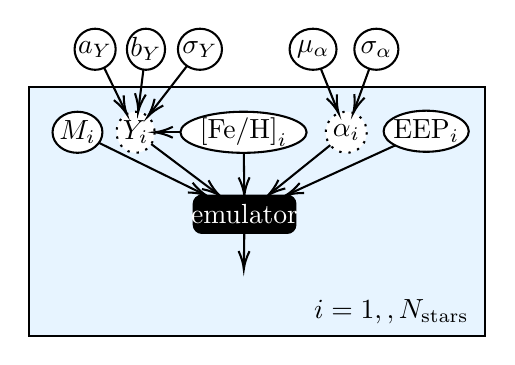
\begin{tikzpicture}[x=0.75pt,y=0.75pt,yscale=-1,xscale=1]
%uncomment if require: \path (0,260); %set diagram left start at 0, and has height of 260

%Shape: Rectangle [id:dp15397896374410736] 
\draw  [fill={rgb, 255:red, 231; green, 244; blue, 255 }  ,fill opacity=1 ][line width=0.75]  (15,40) -- (235,40) -- (235,160) -- (15,160) -- cycle ;

% Text Node
\draw  [fill={rgb, 255:red, 255; green, 255; blue, 255 }  ,fill opacity=1 ][line width=0.75]   (38.5, 62) circle [x radius= 12.02, y radius= 9.9]   ;
\draw (38.5,62) node   [align=left] {$\displaystyle M_{i}$};
% Text Node
\draw  [fill={rgb, 255:red, 255; green, 255; blue, 255 }  ,fill opacity=1 ][line width=0.75]   (206.5, 61.5) circle [x radius= 20.51, y radius= 9.9]   ;
\draw (206.5,61.5) node   [align=left] {$\displaystyle \mathrm{EEP}_{i}$};
% Text Node
\draw  [fill={rgb, 255:red, 0; green, 0; blue, 0 }  ,fill opacity=1 ][line width=0.75]   (94.5,96.5) .. controls (94.5,94.29) and (96.29,92.5) .. (98.5,92.5) -- (139.5,92.5) .. controls (141.71,92.5) and (143.5,94.29) .. (143.5,96.5) -- (143.5,106.5) .. controls (143.5,108.71) and (141.71,110.5) .. (139.5,110.5) -- (98.5,110.5) .. controls (96.29,110.5) and (94.5,108.71) .. (94.5,106.5) -- cycle  ;
\draw (119,101.5) node  [color={rgb, 255:red, 255; green, 255; blue, 255 }  ,opacity=1 ] [align=left] {emulator};
% Text Node
\draw  [fill={rgb, 255:red, 255; green, 255; blue, 255 }  ,fill opacity=1 ][line width=0.75]   (47, 22) circle [x radius= 9.9, y radius= 9.9]   ;
\draw (47,22) node   [align=left] {$\displaystyle a_{Y}$};
% Text Node
\draw  [fill={rgb, 255:red, 255; green, 255; blue, 255 }  ,fill opacity=1 ][line width=0.75]   (71.5, 22) circle [x radius= 9.19, y radius= 9.9]   ;
\draw (71.5,22) node   [align=left] {$\displaystyle b_{Y}$};
% Text Node
\draw  [fill={rgb, 255:red, 255; green, 255; blue, 255 }  ,fill opacity=1 ][line width=0.75]   (97.5, 22) circle [x radius= 10.61, y radius= 9.9]   ;
\draw (97.5,22) node   [align=left] {$\displaystyle \sigma _{Y}$};
% Text Node
\draw  [fill={rgb, 255:red, 255; green, 255; blue, 255 }  ,fill opacity=1 ][dash pattern={on 0.84pt off 2.51pt}][line width=0.75]   (66.5, 62) circle [x radius= 9.19, y radius= 9.9]   ;
\draw (66.5,62) node   [align=left] {$\displaystyle Y_{i}$};
% Text Node
\draw  [fill={rgb, 255:red, 255; green, 255; blue, 255 }  ,fill opacity=1 ][line width=0.75]   (118.5, 62) circle [x radius= 30.41, y radius= 9.9]   ;
\draw (118.5,62) node   [align=left] {$\displaystyle \mathrm{[ Fe/H]}_{i}$};
% Text Node
\draw  [fill={rgb, 255:red, 255; green, 255; blue, 255 }  ,fill opacity=1 ][line width=0.75]   (152, 22) circle [x radius= 11.31, y radius= 9.9]   ;
\draw (152,22) node   [align=left] {$\displaystyle \mu _{\alpha }$};
% Text Node
\draw  [fill={rgb, 255:red, 255; green, 255; blue, 255 }  ,fill opacity=1 ][line width=0.75]   (182.5, 22) circle [x radius= 10.61, y radius= 9.9]   ;
\draw (182.5,22) node   [align=left] {$\displaystyle \sigma _{\alpha }$};
% Text Node
\draw  [fill={rgb, 255:red, 255; green, 255; blue, 255 }  ,fill opacity=1 ][dash pattern={on 0.84pt off 2.51pt}][line width=0.75]   (168, 62) circle [x radius= 9.9, y radius= 9.9]   ;
\draw (168,62) node   [align=left] {$\displaystyle \alpha _{i}$};
% Text Node
\draw (151,141.2) node [anchor=north west][inner sep=0.75pt]   [align=left] {$\displaystyle i=1,\dotsc ,N_{\mathrm{stars}}$};
% Text Node
\draw (111,131.2) node [anchor=north west][inner sep=0.75pt]   [align=left] {$\displaystyle \dotsc $};
% Connection
\draw [line width=0.75]    (51.34,30.9) -- (61.35,51.44) ;
\draw [shift={(62.23,53.23)}, rotate = 244.01] [color={rgb, 255:red, 0; green, 0; blue, 0 }  ][line width=0.75]    (8.74,-2.63) .. controls (5.56,-1.12) and (2.65,-0.24) .. (0,0) .. controls (2.65,0.24) and (5.56,1.12) .. (8.74,2.63)   ;
% Connection
\draw [line width=0.75]    (70.27,31.81) -- (67.97,50.2) ;
\draw [shift={(67.73,52.19)}, rotate = 277.13] [color={rgb, 255:red, 0; green, 0; blue, 0 }  ][line width=0.75]    (8.74,-2.63) .. controls (5.56,-1.12) and (2.65,-0.24) .. (0,0) .. controls (2.65,0.24) and (5.56,1.12) .. (8.74,2.63)   ;
% Connection
\draw [line width=0.75]    (91.28,30.02) -- (73.62,52.82) ;
\draw [shift={(72.39,54.4)}, rotate = 307.78] [color={rgb, 255:red, 0; green, 0; blue, 0 }  ][line width=0.75]    (8.74,-2.63) .. controls (5.56,-1.12) and (2.65,-0.24) .. (0,0) .. controls (2.65,0.24) and (5.56,1.12) .. (8.74,2.63)   ;
% Connection
\draw [line width=0.75]    (155.74,31.35) -- (163.58,50.95) ;
\draw [shift={(164.32,52.81)}, rotate = 248.2] [color={rgb, 255:red, 0; green, 0; blue, 0 }  ][line width=0.75]    (8.74,-2.63) .. controls (5.56,-1.12) and (2.65,-0.24) .. (0,0) .. controls (2.65,0.24) and (5.56,1.12) .. (8.74,2.63)   ;
% Connection
\draw [line width=0.75]    (179.1,31.38) -- (172.06,50.81) ;
\draw [shift={(171.37,52.69)}, rotate = 289.93] [color={rgb, 255:red, 0; green, 0; blue, 0 }  ][line width=0.75]    (8.74,-2.63) .. controls (5.56,-1.12) and (2.65,-0.24) .. (0,0) .. controls (2.65,0.24) and (5.56,1.12) .. (8.74,2.63)   ;
% Connection
\draw [line width=0.75]    (191.61,68.31) -- (140.51,91.67) ;
\draw [shift={(138.69,92.5)}, rotate = 335.43] [color={rgb, 255:red, 0; green, 0; blue, 0 }  ][line width=0.75]    (8.74,-2.63) .. controls (5.56,-1.12) and (2.65,-0.24) .. (0,0) .. controls (2.65,0.24) and (5.56,1.12) .. (8.74,2.63)   ;
% Connection
\draw [line width=0.75]    (48.83,67.07) -- (98.86,91.62) ;
\draw [shift={(100.66,92.5)}, rotate = 206.14] [color={rgb, 255:red, 0; green, 0; blue, 0 }  ][line width=0.75]    (8.74,-2.63) .. controls (5.56,-1.12) and (2.65,-0.24) .. (0,0) .. controls (2.65,0.24) and (5.56,1.12) .. (8.74,2.63)   ;
% Connection
\draw [line width=0.75]    (74.04,67.67) -- (105.44,91.3) ;
\draw [shift={(107.04,92.5)}, rotate = 216.96] [color={rgb, 255:red, 0; green, 0; blue, 0 }  ][line width=0.75]    (8.74,-2.63) .. controls (5.56,-1.12) and (2.65,-0.24) .. (0,0) .. controls (2.65,0.24) and (5.56,1.12) .. (8.74,2.63)   ;
% Connection
\draw [line width=0.75]    (160.29,68.21) -- (131.72,91.24) ;
\draw [shift={(130.16,92.5)}, rotate = 321.13] [color={rgb, 255:red, 0; green, 0; blue, 0 }  ][line width=0.75]    (8.74,-2.63) .. controls (5.56,-1.12) and (2.65,-0.24) .. (0,0) .. controls (2.65,0.24) and (5.56,1.12) .. (8.74,2.63)   ;
% Connection
\draw    (118.63,71.9) -- (118.86,90.5) ;
\draw [shift={(118.89,92.5)}, rotate = 269.27] [color={rgb, 255:red, 0; green, 0; blue, 0 }  ][line width=0.75]    (8.74,-2.63) .. controls (5.56,-1.12) and (2.65,-0.24) .. (0,0) .. controls (2.65,0.24) and (5.56,1.12) .. (8.74,2.63)   ;
% Connection
\draw    (118.87,110.5) -- (118.65,126) ;
\draw [shift={(118.63,128)}, rotate = 270.81] [color={rgb, 255:red, 0; green, 0; blue, 0 }  ][line width=0.75]    (8.74,-2.63) .. controls (5.56,-1.12) and (2.65,-0.24) .. (0,0) .. controls (2.65,0.24) and (5.56,1.12) .. (8.74,2.63)   ;
% Connection
\draw    (88.09,62) -- (77.69,62) ;
\draw [shift={(75.69,62)}, rotate = 360] [color={rgb, 255:red, 0; green, 0; blue, 0 }  ][line width=0.75]    (8.74,-2.63) .. controls (5.56,-1.12) and (2.65,-0.24) .. (0,0) .. controls (2.65,0.24) and (5.56,1.12) .. (8.74,2.63)   ;

\end{tikzpicture}
